\documentclass[a4paper, 11pt]{article}

\usepackage[slovene]{babel}
\usepackage[utf8]{inputenc}
\usepackage[T1]{fontenc}
\usepackage{lmodern}
\usepackage{amsmath}
\usepackage{amsfonts}
\usepackage{amssymb}
\usepackage{enumitem}
\usepackage{epsdice}
\usepackage{array}
\usepackage[table]{xcolor}
\usepackage{makecell}
\usepackage{hyperref}

\usepackage{geometry}
\geometry{
 a4paper,
 total={170mm,257mm},
 left=25mm,
 top=25mm,
 }

\newcolumntype{P}[1]{>{\centering\arraybackslash}p{#1}}

\begin{document}

\title{\textbf{\LARGE{Model napovedi odjema električne energije}} \\ Matematika z računalnikom 2023/24}
\author{Karolina Šavli}
\date{Maj 2024}

\maketitle

% =======================================================================================================================
% =======================================================================================================================


\section{Uvod}

Cilj projektne naloge je sestaviti model, ki bo napovedal odjem električne energije 
za celotni naslenji dan (za naslednjih $24$ ur). 



% =======================================================================================================================
% =======================================================================================================================


\section{Osnovna analiza časovne vrste}

\noindent Podjetje GEN-I je v obliki excel razpredelnice pripravilo tabelo podatkov, sestavljeno iz sedmih stolpcev:
\begin{itemize}
    \item  \texttt{DateTimeStartUTC}: univerzalni koordinirani čas,
    \item  \texttt{DateTimeStartCET}: srednjeevropski čas,
    \item  \texttt{Odjem ACT}: neto odjem električne energije v kWh,
    \item  \texttt{Temperatura ACT}: dejanska temperatura, 
    \item  \texttt{Temperatura FC}: napovedana temperatura,
    \item  \texttt{Sevanje ACT}: dejansko sevanje in
    \item  \texttt{Sevanje FC}: napovedano sevanje. 
\end{itemize}

\begin{figure}[h!]
    \centering
    \caption{Tabela podatkov, 2021-2024}\par\medskip
    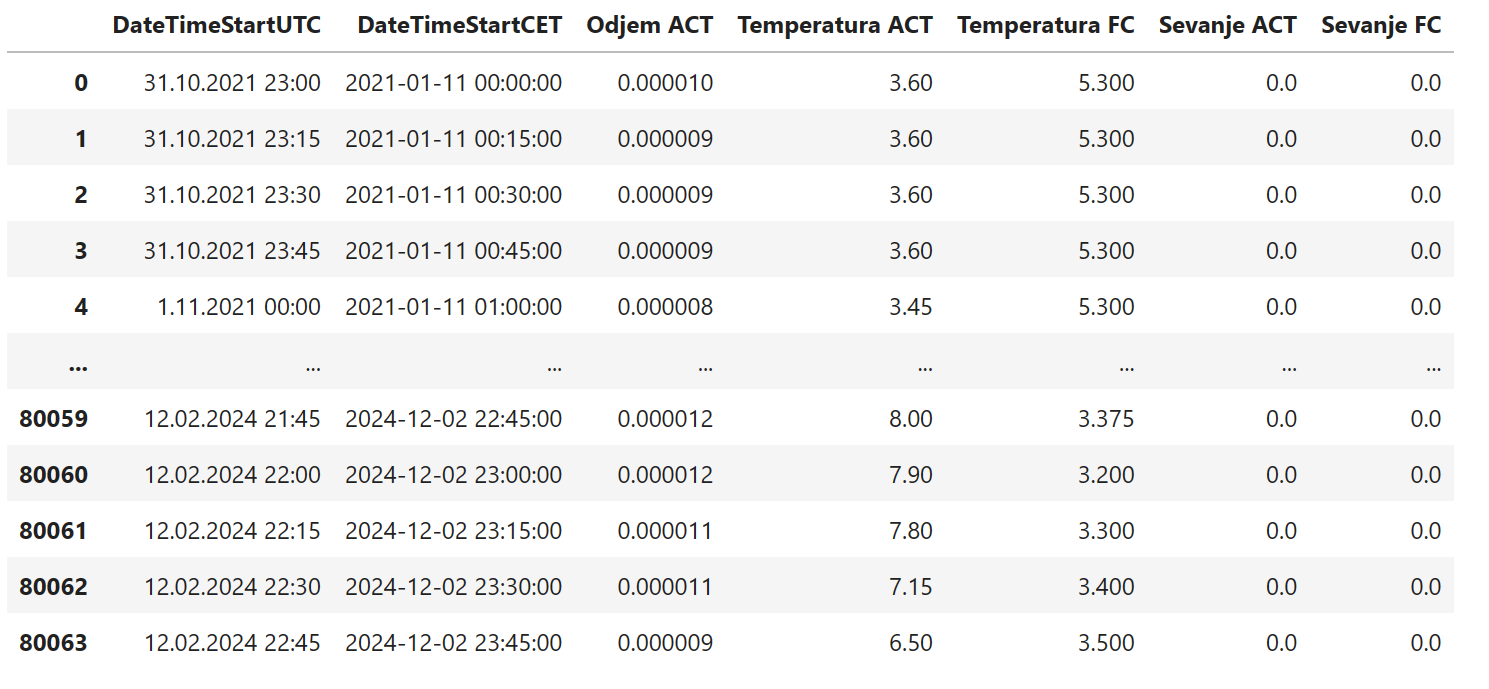
\includegraphics[width=0.9\textwidth]{tabela.png}
\end{figure}

\noindent V analizi sem uporabljala vse stolpce, razen stolpca \texttt{DateTimeStartUTC}, saj je v 
okviru časa bolj relavanten stolpec \texttt{DateTimeStartCET}. Podatki so podani za odboje od $1.~\text{novembra}~2021$ do $12.~\text{februarja}~2024$,
na vsakih $15$ minut. Tabela ima torej vsega skupaj $80064$ vrstic. \\

\begin{figure}[h!]
    \centering
    \caption{Odjem električne energije, 2021-2024}\par\medskip
    \label{fig:odjem_EE}
    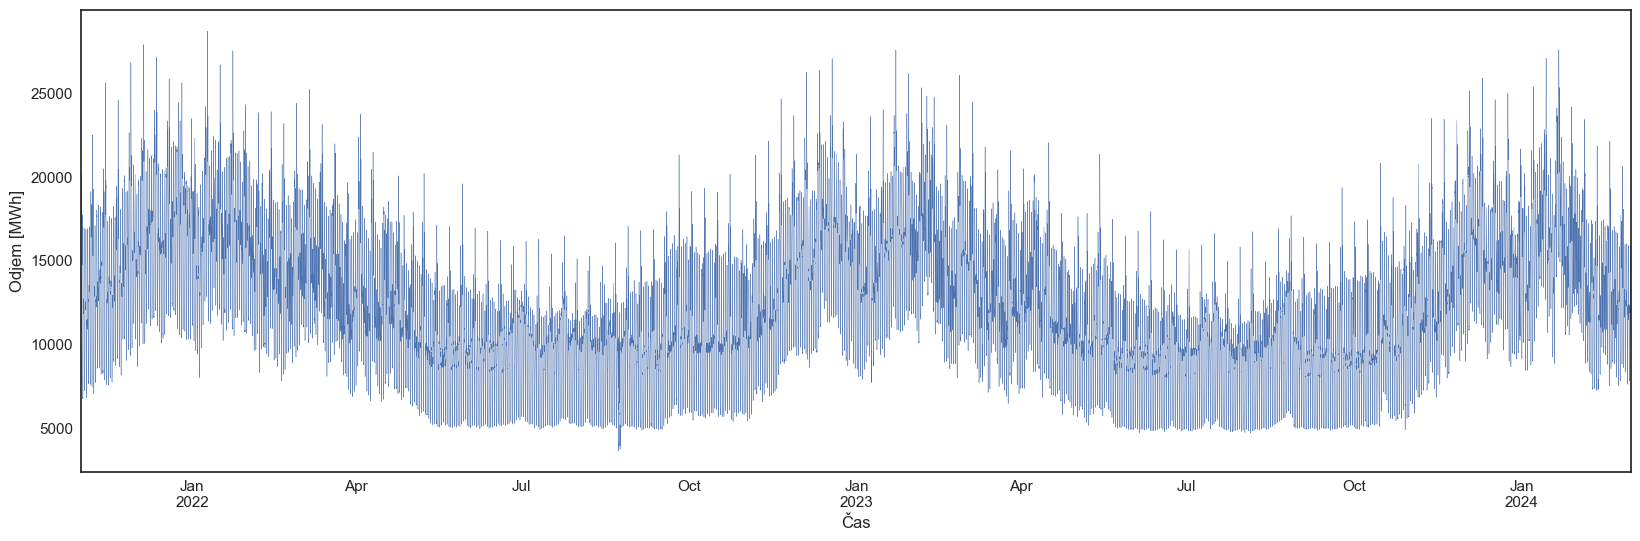
\includegraphics[width=0.9\textwidth]{odjem_EE.png}
\end{figure}

\noindent Slika~\ref{fig:odjem_EE} prikazuje odjem električne energije za obdobje od 
$1.~\text{novembra}~2021$ do $12.~\text{februarja}~2024$. 
Opaznoa je sezonskost; odjem je znatno večji jeseni in pozimi, zaradi povečane uporabe energije za ogrevanje in 
razsvetljevo, saj se število ur dnevne svetlobe podaljša. 

\begin{table}[!h]
    \centering
    \caption{Opisne statistike porabe električne energije, 2021-2024}\par\medskip
    \label{Tab:opisne_statistike}
    \begin{tabular}{l||l|l|l|l|l}
              & Min & Max & Povprečje & Mediana & Standardni odklon \\ \hline \hline
        Odjem [MWh] & 3629,32 & 28736,80 & 12240,53 & 11708,50 & 4167,98 \\ 
    \end{tabular}
\end{table}

\noindent S Tabele~\ref{Tab:opisne_statistike} preberemo, da je povprečna poraba električne energije gospodinjskih odjemalcev
okrog $12240{,}53 $ MWh, minimalna dosežena vrednost je $3629{,}32$ MWh, maksimalna pa $28736{,}80$ MWh. Vrednosti varirajo
okrog $4167{,}98$ MWh. \\

\noindent Odjem električne energije je med tednom najmanjši ponoči in se veča do viška okrog 18 ure. 
V soboto in nedeljo pa je prvi višek porabe dopoldne, drugi pa okrog 18 ure, kar je opazno s Slike~\ref{fig:odjem_teden}, ki prikazuje odjem 
električne energije v drugem tednu septembra 2023. \\

\begin{figure}[h!]
    \centering
    \caption{Odjem električne energije po dneh, drugi teden septembra 2023}\par\medskip
    \label{fig:odjem_teden}
    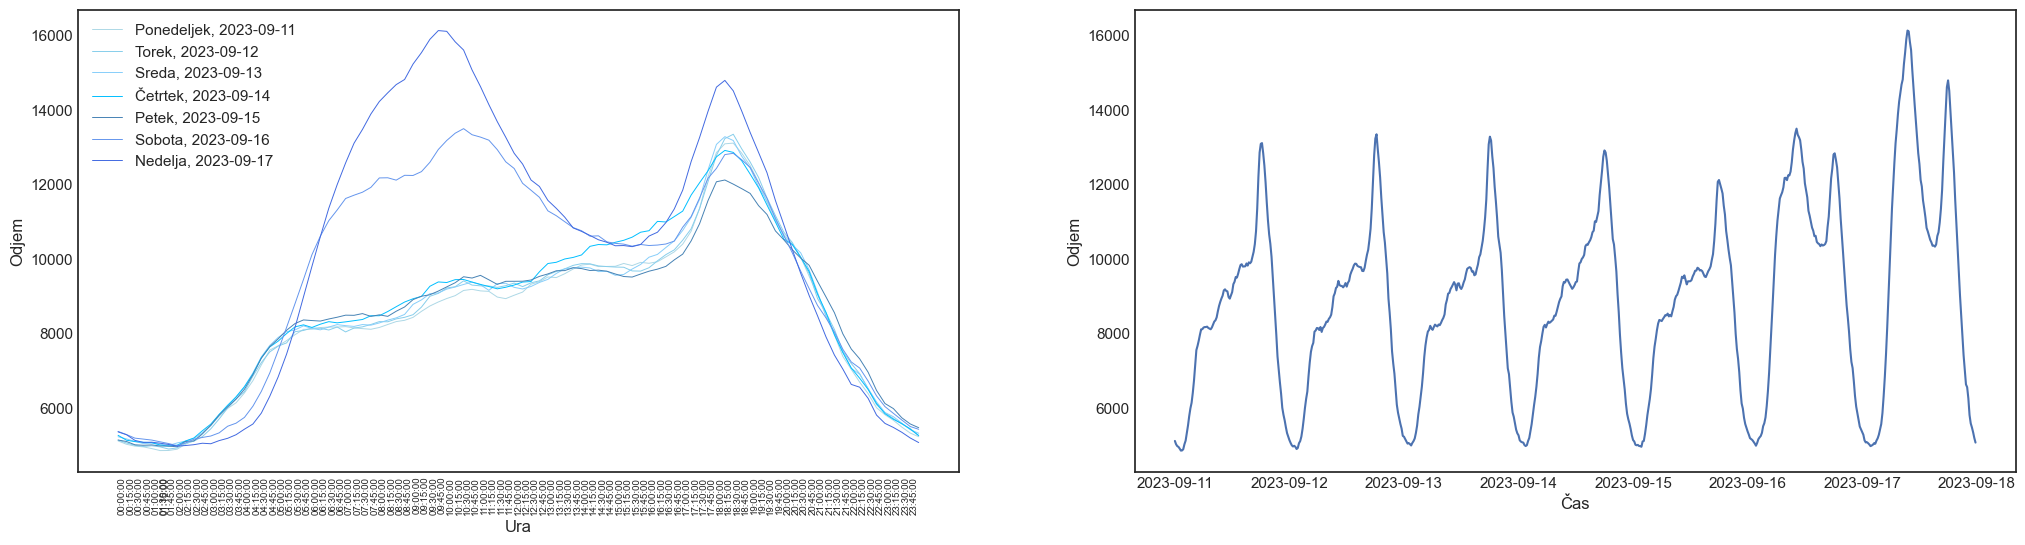
\includegraphics[width=0.9\textwidth]{odjem_teden.png}
\end{figure}






% =======================================================================================================================
% =======================================================================================================================


\section{Napredna analiza}



% =======================================================================================================================
% =======================================================================================================================


\section{Izbira modela}



% =======================================================================================================================
% =======================================================================================================================


\section{Zaključek}



% =======================================================================================================================
% =======================================================================================================================


\end{document}
